\let\lesson\undefined
\newcommand{\lesson}{\phantomlesson{Bài 10.}}
\let\lesson\undefined
\newcommand{\lesson}{\phantomlesson{Bài 10.}}


\setcounter{section}{2}
\section{Trắc nghiệm}
\setcounter{ex}{0}
\Opensolutionfile{ans}[ans/VN12-Y24-PH-SYL-019P-TN]
% ===================================================================
\begin{ex}\mkstar{1}
	Phát biểu nào sau đây \textbf{đúng}?
	\choice
	{Hai dòng điện thẳng song song ngược chiều hút nhau, cùng chiều đẩy nhau}
	{Dòng điện không tương tác với dòng điện}
	{\True Hai dòng điện thẳng song song cùng chiều hút nhau, ngược chiều đẩy nhau}
	{Dòng điện và nam châm không tương tác với nhau}
	\loigiai{}
\end{ex}
% ===================================================================
\begin{ex}\mkstar{1}
Độ lớn cảm ứng từ tại một điểm cách dòng điện thẳng dài vô hạn một đoạn $r$ (với $I$ là cường độ dòng điện trong dây dẫn) là
	\choice
	{$B=2 \cdot 10^{-7}\cdot\dfrac{I}{r^2}$}
	{$B=2 \cdot 10^7 \cdot\dfrac{I}{r}$}
	{\True $B=2 \cdot 10^{-7} \dfrac{I}{r}$}
	{$B=4 \pi \cdot 10^{-7} \cdot\dfrac{I}{r}$}
	\loigiai{}
\end{ex}
% ===================================================================
\begin{ex}\mkstar{1}
	Độ lớn cảm ứng từ tại tâm dòng điện tròn có $N$ vòng dây và có bán kính $R$ (với $I$ là cường độ dòng điện trong dây dẫn) là
	\choice
	{$B=2 \cdot 10^{-7} \cdot\dfrac{NI}{R}$}
	{\True $B=2 \pi \cdot 10^{-7}\cdot \dfrac{NI}{R}$}
	{$B=2 \pi \cdot 10^7 \cdot\dfrac{NI}{R}$}
	{$B=4 \pi \cdot 10^{-7}\cdot \dfrac{NI}{R}$}
	\loigiai{}
\end{ex}
% ===================================================================
\begin{ex}\mkstar{1}
	Độ lớn cảm ứng từ bên trong ống dây có chiều dài $L$ và $N$ vòng dây (chiều dài ống dây rất lớn so với bán kính vòng dây) với $I$ là cường độ dòng điện trong dây dẫn là
	\choice
	{$B=2 \cdot 10^{-7} \cdot\dfrac{NI}{L}$}
	{$B=2 \pi \cdot 10^{-7} \cdot\dfrac{NI}{L}$}
	{\True $B=4 \pi \cdot 10^{-7}\cdot \dfrac{NI}{L}$}
	{$B=4 \pi \cdot 10^7\cdot \dfrac{NI}{L}$}
	\loigiai{}
\end{ex}

% ===================================================================
\begin{ex}\mkstar{2}
	Biết độ lớn cảm ứng từ do một dây dẫn thẳng dài mang dòng điện $I$ tạo ra ở vị trí cách trục dây dẫn một khoảng $r$ là $B=2,0 \cdot 10^{-7}\cdot \dfrac{I}{r}$, với $B$ tính bằng tesla $\left(\si{\tesla}\right)$, $r$ tính bằng mét $\left(\si{\meter}\right)$ và $I$ tính bằng ampere $\left(\si{\ampere}\right)$.\\
	Một dây dẫn thẳng dài $\SI{2}{\meter}$ mang dòng điện $\SI{10}{\ampere}$. Độ lớn cảm ứng từ do dòng điện gây ra ở vị trí cách nó $\SI{2}{\centi\meter}$ lớn gấp mấy lần so với ở khoảng cách $\SI{4}{\centi\meter}$?
	\choice
	{\True 2}
	{$2 \sqrt{2}$}
	{4}
	{$4 \sqrt{2}$}
	\loigiai{
$$\dfrac{B_1}{B_2}=\dfrac{r_2}{r_1}=2.$$	
}
\end{ex}
% ===================================================================
\begin{ex}\mkstar{2}
Hai dây dẫn thẳng, rất dài, đặt song song, cách nhau $\SI{20}{\centi\meter}$ trong không khí, có hai dòng điện ngược chiều, có cường độ $I_1 =\SI{12}{\ampere}$; $I_2 =\SI{15}{\ampere}$ chạy qua. Độ lớn cảm ứng từ tổng hợp do hai dòng điện này gây ra tại điểm M cách dây dẫn mang dòng $I_1$ một đoạn $\SI{15}{\centi\meter}$ và cách dây dẫn mang dòng $I_2$ một đoạn $\SI{5}{\centi\meter}$ là
	\choice
	{$\SI{1.6E-5}{\tesla}$}
	{$\SI{6E-5}{\tesla}$}
	{\True $\SI{7.6E-5}{\tesla}$}
	{$\SI{4.4E-5}{\tesla}$}
	\loigiai{
Hai dòng điện gây ra cảm ứng từ tại M như hình vẽ:
\begin{center}
	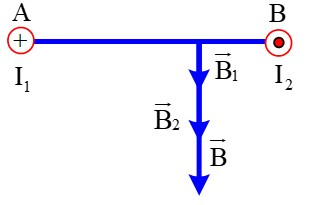
\includegraphics[width=0.25\linewidth]{../figs/VN12-Y24-PH-SYL-019P-4}
\end{center}	
Độ lớn cảm ứng từ do mỗi dòng điện gây ra tại M:
$$\begin{cases}
	B_1=\SI{2E-7}{}\cdot\frac{I_1}{\mathrm{AM}}=\SI{1.6E-5}{\tesla}\\
	B_2=\SI{2E-7}{}\cdot\dfrac{I_2}{\mathrm{BM}}=\SI{6E-5}{\tesla}
\end{cases}$$
Cảm ứng từ tổng hợp tại M:
$$\vec{B}_{\mathrm{M}}=\vec{B}_1+\vec{B}_2.$$
Vì $\vec{B}_1\uparrow\uparrow\vec{B}_2$ nên độ lớn cảm ứng từ tổng hợp tại M:
$$B_\mathrm{M}=B_1+B_2=\SI{7.6E-5}{\tesla}.$$
}
\end{ex}
% ===================================================================
\begin{ex}\mkstar{2}
	Cuộn dây tròn dẹt có 20 vòng, bán kính là $\SI{3.14}{\centi\meter}$. Khi có dòng điện đi vào thì tại tâm của vòng dây xuất hiện từ trường là $B =\SI{2}{\milli\tesla}$. Cường độ dòng điện trong vòng dây là
	\choice
	{$\SI{3}{\ampere}$}
	{$\SI{4}{\ampere}$}
	{\True $\SI{5}{\ampere}$}
	{$\SI{2.5}{\ampere}$}
	\loigiai{
Cường độ dòng điện trong vòng dây là
$$B=2\pi\cdot10^{-7}\cdot\dfrac{NI}{R}\Rightarrow I=\dfrac{BR}{2\pi\cdot 10^{-7}N}=\dfrac{2\cdot 10^{-3}\cdot 3,14\cdot10^{-2}}{40\pi\cdot10^{-7}}=\SI{5}{\ampere}.$$
}
\end{ex}
% ===================================================================
\begin{ex}\mkstar{2}
	Một dây dẫn đường kính tiết diện $d =\SI{0.5}{\milli\meter}$ được phủ một lớp sơn cách điện mỏng và quấn thành một ống dây, các vòng dây quấn sát nhau. Cho dòng điện có cường độ $I =\SI{2}{\ampere}$ chạy qua ống dây. Độ lớn cảm ứng từ tại một điểm trên trục trong ống dây là
	\choice
	{\True $\SI{5E-3}{\tesla}$}
	{$\SI{2.5E-4}{\tesla}$}
	{$\SI{1.25E-4}{\tesla}$}
	{$\SI{3.75E-4}{\tesla}$}
	\loigiai{
\begin{itemize}
	\item Số vòng dây quấn sát nhau trên ống dây: $N=\dfrac{\ell}{d}$.
	\item Cảm ứng từ tại một điểm bên trong ống dây: $$B=4\pi \cdot 10^{-7}\cdot\dfrac{I}{d}=\SI{5E-3}{\tesla}.$$
\end{itemize}	
}
\end{ex}
% ===================================================================
\begin{ex}\mkstar{2}
	Cho dòng điện cường độ $I = \SI{0.15}{\ampere}$ chạy qua các vòng dây của một ống dây, thì cảm ứng từ bên trong ống dây là $B =\SI{35E-5}{\tesla}$. Ống dây dài $\SI{50}{\centi\meter}$. Lấy $\pi=3,14$. Số vòng dây của ống dây là
	\choice
	{1858 vòng}
	{\True 929 vòng}
	{1394 vòng}
	{465 vòng}
	\loigiai{
Cảm ứng từ bên trong ống dây: $B=4\pi\cdot10^{-7}\dfrac{N}{\ell}I$.\\
Số vòng dây của ống dây:
$$N=\dfrac{\ell B}{4\pi\cdot10^{-7}I}=\SI{929}{\text{vòng}}.$$	
}
\end{ex}
% ===================================================================
\begin{ex}\mkstar{3}
	Dùng một dây đồng có phủ một lớp sơn cách điện mỏng, quấn quanh một hình trụ dài $L = \SI{60}{\centi\meter}$, có đường kính $d =\SI{3}{\centi\meter}$ để làm một ống dây. Sợi dây quấn có chiều dài $\ell = \SI{314}{\centi\meter}$ và các vòng dây được quấn sát nhau. Lấy $\pi=3,14$ Nếu cho dòng điện cường độ $I = \SI{0.5}{\ampere}$ chạy qua ống dây, thì cảm ứng từ bên trong ống dây có độ lớn \textbf{gần nhất} với giá trị nào?
	\choice
	{$\SI{5E-5}{\tesla}$}
	{$\SI{2.5E-5}{\tesla}$}
	{$\SI{1.25E-5}{\tesla}$}
	{\True $\SI{3.5E-5}{\tesla}$}
	\loigiai{
\begin{itemize}
	\item Chu vi mỗi vòng dây: $\pi d$
	\item Số vòng dây: $N=\dfrac{\ell}{\pi d}$
	\item Cảm ứng từ bên trong ống dây:
	$$B=4\pi\cdot10^{-7}\dfrac{N}{L}I=\SI{3.5E-5}{\tesla}.$$
\end{itemize}	
}
\end{ex}

% ===================================================================
\begin{ex}\mkstar{3}
	Hai dây dẫn thẳng, rất dài, đặt song song, cách nhau $\SI{20}{\centi\meter}$ trong không khí, có hai dòng điện ngược chiều, có cường độ $I_1=I_2=\SI{12}{\ampere}$ chạy qua. Độ lớn cảm ứng từ tổng hợp do hai dòng điện này gây ra tại điểm M cách dây dẫn mang dòng điện $I_1$ đoạn $\SI{16}{\centi\meter}$ và cách dây dẫn mang dòng $I_2$ đoạn $\SI{12}{\centi\meter}$ là
	\choice
	{$\SI{1.5E-5}{\tesla}$}
	{$\SI{2E-5}{\tesla}$}
	{\True $\SI{2.5E-5}{\tesla}$}
	{$\SI{3.5E-5}{\tesla}$}
	\loigiai{
		Tam giác AMB vuông tại M.\\
		Các dòng điện $I_1$ và $I_2$ gây ra tại M các vector cảm ứng từ $B_1$ và $B_2$ có phương chiều như hình vẽ:
		\begin{center}
			\begin{tikzpicture}
				\coordinate (A) at (0,0);
				\coordinate (B) at (4,0);
				\coordinate (M) at (3,-1.732);
				\coordinate (C) at ($(M)+(-30:2)$);
				\coordinate (D) at ($(M)+(-120:2.5)$);
				\coordinate (E) at ($(C)+(-120:2.5)$);
				\draw[line width=1.5pt, blue] (A)--(B)--(M)--(A);
				\draw[-stealth, teal, line width=1.5pt] (M)--(D);
				\draw[-stealth, teal, line width=1.5pt] (M)--(C);
				\draw[dashed, red, line width=1pt] (D)--+(-30:2);
				\draw[dashed, red, line width=1pt] (C)--+(-120:2.5);
				\draw[-stealth, red, line width=1.5pt] (M)--(E);
				\node[right, teal] at (C) {$\vec{B}_2$};
				\node[left, teal] at (D) {$\vec{B}_1$};
				\node[below, red] at (E) {$\vec{B}$};
				\fill[red] (M) circle [radius=3pt] node[right] {M};
				\node[red, line width=2pt, fill=white, inner sep=0pt] at (A) {\LARGE$\otimes$};
				\node[red, line width=2pt, fill=white, inner sep=0pt] at (B) {\LARGE$\odot$};
				\node[above] at (0,0.25) {A};
				\node[above] at (4,0.25) {B};
				\node[below] at (0,-0.25) {$I_1$};
				\node[below] at (4,-0.25) {$I_2$};
			\end{tikzpicture}
		\end{center}	
	Độ lớn các vector cảm ứng từ thành phần:
	$$
	\begin{cases}
		B_1=\SI{2E-7}{}\cdot\frac{I_1}{\mathrm{AM}}=\SI{1.5E-5}{\tesla}\\
		B_2=\SI{2E-7}{}\cdot\frac{I_2}{\mathrm{BM}}=\SI{2E-5}{\tesla}
	\end{cases}$$
Cảm ứng từ tổng hợp tại M có độ lớn:
$$B_{\mathrm{M}}=\sqrt{B^2_1+B^2_2}=\SI{2.5E-5}{\tesla}.$$
}
\end{ex}

% ===================================================================
\begin{ex}\mkstar{3}
	Cho hai dây dẫn thẳng dài vô hạn đặt song song cách nhau một đoạn bằng $\SI{32}{\centi\meter}$, dòng điện chạy qua các dây dẫn có cường độ lần lượt là $I_1=\SI{0.1}{\ampere}$ và $I_2$. Xét một mặt phẳng vuông góc với mặt phẳng tạo bởi hai dây dẫn, mặt phẳng này cắt hai dây dẫn $I_1$ và $I_2$ lần lượt tại hai điểm A và B. Xét điểm M nằm trên đường nối AB và nằm ngoài AB, biết $AM=\SI{8}{\centi\meter}$. Để cảm ứng từ tại M bị triệt tiêu thì dòng điện $I_2$ có cường độ và chiều thỏa mãn:	 
	\choice
	{\True cường độ $I_2=\SI{0.5}{\ampere}$ và ngược chiều với $I_1$}
	{cường độ $I_2=\SI{0.8}{\ampere}$ và cùng chiều với $I_1$}
	{cường độ $I_2=\SI{0.5}{\ampere}$ và cùng chiều với $I_1$}
	{cường độ $I_2=\SI{0.8}{\ampere}$ và ngược chiều với $I_1$}
	\loigiai{
		Do điểm M nằm ngoài khoảng giữa hai dây dẫn nên dòng điện $I_2$ phải ngược chiều với dòng điện $I_1$. Giả sử hai dòng điện có chiều như hình vẽ:
		\begin{center}
			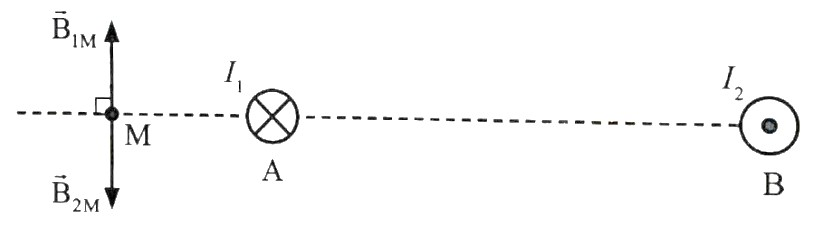
\includegraphics[width=0.4\linewidth]{../figs/VN12-Y24-PH-SYL-018P-2}
		\end{center}	
		$$
		B_{1 M}=B_{2 \mathrm{M}} \Rightarrow 2\cdot10^{-7} \frac{I_1}{A M}=2\cdot10^{-7} \frac{I_2}{BM} \Rightarrow I_2=I_1 \frac{BM}{AM}=0,1 \cdot \frac{40\cdot10^{-2}}{8\cdot10^{-2}}=\SI{0.5}{\ampere}.
		$$
	}
\end{ex}
% ===================================================================
\begin{ex}\mkstar{3}
	Một dây dẫn thẳng, dài có vỏ bọc cách điện, ở khoảng giữa được uốn thành vòng tròn, bán kính $R =\SI{20}{\centi\meter}$ như hình vẽ. Dòng điện chạy qua dây dẫn có cường độ $\SI{5}{\ampere}$. Độ lớn cảm ứng từ tại tâm O của vòng tròn là
	\begin{center}
		\begin{tikzpicture}
			\draw[line width=2pt, color=purple, decoration={markings, mark=at position 0.5 with {\arrowreversed{stealth}}},
			postaction={decorate}
			] (0,0 )circle (1.5);
			\draw[purple, line width=2pt,decoration={markings, mark=at position 0.25 with {\arrow{stealth}}},
			postaction={decorate}
			] (-3,-1.5)--(3,-1.5);
			\draw[line width=3pt, color=white] (-0.25,-1.5)--(0.25,-1.5);
			\node[above] at (-1.5,-1.5) {$I$};
			\fill[black] (0,0) circle [radius=2pt] node[above] {O};
		\end{tikzpicture}
	\end{center}
	\choice
	{$\SI{5E-6}{\tesla}$}
	{$\SI{15.7E-6}{\tesla}$}
	{\True $\SI{10.7E-6}{\tesla}$}
	{$\SI{20.7E-6}{\tesla}$}
	\loigiai{
Cảm ứng từ do hai dòng điện gây ra tại O được biểu diễn như hình bên dưới:
\begin{center}
	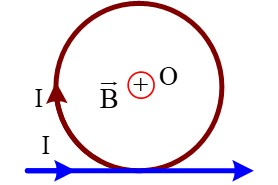
\includegraphics[width=0.2\linewidth]{../figs/VN12-Y24-PH-SYL-019P-7}
\end{center}	
Độ lớn cảm ứng từ do mỗi dòng điện gây ra tại O:
$$\begin{cases}
	B_1=2\pi\cdot10^{-7}\cdot\dfrac{I}{R}=\SI{15.7E-6}{\tesla}\\
	B_2=\SI{2E-7}{}\cdot\dfrac{I}{R}=\SI{5E-6}{\tesla}
\end{cases}
$$
Vì $\vec{B}_1\uparrow\downarrow\vec{B}_2$ nên độ lớn cảm ứng từ tổng hợp:
$$B=\left|B_1-B_2\right|=\SI{10.7E-6}{\tesla}.$$
}
\end{ex}

% ===================================================================
\begin{ex}\mkstar{3}
Một dòng điện thẳng dài có $I=\SI{100}{\ampere}$ đặt trong một từ trường dều $B_0=\SI{5E-4}{\tesla}$. Dây dẫn vuông góc với đường cảm ứng từ của từ trường đều. Điểm có cảm ứng từ tổng hợp bằng 0 cách dây dẫn một đoạn
	\choice
	{$\SI{6}{\centi\meter}$}
	{\True $\SI{4}{\centi\meter}$}
	{$\SI{8}{\centi\meter}$}
	{$\SI{2}{\centi\meter}$}
	\loigiai{
$$\vec{B}_0+\vec{B}=\vec{0}\Rightarrow B=B_0\Rightarrow \SI{5E-4}{}=\SI{2E-7}{}\cdot\dfrac{100}{r}\Rightarrow r=\SI{0.04}{\meter}.$$	
}
\end{ex}

% ===================================================================
\begin{ex}\mkstar{3}
	Hai dây dẫn thẳng, rất dài, đặt song song, cách nhau $\SI{10}{\centi\meter}$ trong không khí, có hai dòng điện cùng chiều, cùng cường độ $I_1=I_2=\SI{6}{\ampere}$ chạy qua. Độ lớn cảm ứng từ tổng hợp do hai dòng điện này gây ra tại điểm M cách đều hai dây dẫn một khoảng $\SI{20}{\centi\meter}$ là
	\choice
	{$\SI{6E-6}{\tesla}$}
	{\True $\SI{11.6E-6}{\tesla}$}
	{$\SI{5E-6}{\tesla}$}
	{$\SI{12E-6}{\tesla}$}
	\loigiai{
Các dòng điện $I_1$ và $I_2$ gây ra cảm ứng từ tại M như hình vẽ:
\begin{center}
	\begin{tikzpicture}
		\coordinate (M) at (0,0);
		\coordinate (A) at ($(M)+(70:4)$);
		\coordinate (B) at ($(M)+(110:4)$);
		\coordinate (H) at ($(A)!(M)!(B)$);
		\coordinate (B2) at ($(M)+(160:2)$);
		\coordinate (B1) at ($(M)+(200:2)$);
		\coordinate (B0) at ($(B2)+(200:2)$);
		\draw[line width=2pt, blue] (A)--(B)--(M)--(A);
		\draw[-stealth, teal, line width=2pt] (M)--(B1);
		\draw[-stealth, teal, line width=2pt] (M)--(B2);
		\draw[-stealth, red, line width=2pt] (M)--(B0);
		\draw[dashed, red, line width=1.5pt] (B1)--(B0)--(B2);
		\draw[dashed, blue, line width=1.5pt] (M)--(H);
		\node[red, fill=white, inner sep=0pt] at (A) {\LARGE$\otimes$};
		\node[red, fill=white, inner sep=0pt] at (B) {\LARGE$\otimes$};
		\fill[red] (M) circle [radius=2.5pt] node[right] {M};
		\node[above] at ($(A)+(0,0.25)$) {$I_2$};
		\node[above] at ($(B)+(0,0.25)$) {$I_1$};
		\node[below] at ($(B)+(0,-0.25)$) {A};
		\node[below] at ($(A)+(0,-0.25)$) {B};
		\node[below] at (B1) {$\vec{B}_1$};
		\node[above] at (B2) {$\vec{B}_2$};
		\node[left] at (B0) {$\vec{B}$};
		\node[above] at (H) {H};
		\tkzMarkAngle[size=0.75cm,color=red, line width=1.5pt](A,M,H);
		\tkzLabelAngle[color=black,pos=1.2](A,M,H){$\alpha$};
		\tkzMarkAngle[size=0.75cm,color=red,line width=1.5pt](H,M,B);
		\tkzLabelAngle[color=black,pos=1.2](H,M,B){$\alpha$};
		\tkzMarkAngle[size=0.75cm,color=red, line width=1.5pt](B2,M,B0);
		\tkzLabelAngle[color=black,pos=1.2](B2,M,B0){$\alpha$};
		\tkzMarkAngle[size=0.75cm,color=red,line width=1.5pt](B0,M,B1);
		\tkzLabelAngle[color=black,pos=1.2](B0,M,B1){$\alpha$};
	\end{tikzpicture}
\end{center}	
Độ lớn cảm ứng từ do mỗi dòng điện gây ra tại M:
$$B_1=B_2=\SI{2E-7}{}\cdot\dfrac{I_1}{\mathrm{AM}}=\SI{6E-6}{\tesla}.$$
Độ lớn cảm ứng từ tổng hợp tại M:
$$B=2B_1\cos\alpha=2B_1\dfrac{\sqrt{\mathrm{AM}^2-\mathrm{AH}^2}}{\mathrm{AM}}=\SI{11.6E-6}{\tesla}.$$
}
\end{ex}
%% ===================================================================
%\begin{ex}\mkstar{3}
%	Một dây dẫn trong không khí được uốn thành vòng tròn bán kính $R =\SI{0.1}{\meter}$, có dòng điện $I =\SI{3.2}{\ampere}$ chạy qua. Mặt phẳng vòng dây trùng với mặt phẳng kinh tuyến từ. Tại tâm vòng dây treo một kim nam châm nhỏ. Tính góc quay của kim nam châm khi ngắt dòng điện. Cho biết thành phần nằm ngang của cảm ứng từ Trái Đất có $B_d =\SI{2E-5}{\tesla}$.
%	\choice
%	{\True $\SI{44.85}{\degree}$}
%	{$\SI{30}{\degree}$}
%	{$\SI{60}{\degree}$}
%	{$\SI{90}{\degree}$}
%	\loigiai{
%\begin{itemize}
%	\item Cảm ứng từ gây ra bởi dòng điện tại tâm vòng dây có phương vuông góc với mặt phẳng vòng dây, suy ra nó cũng vuông góc với cảm ứng từ của Trái Đất $\rightarrow \vec{B}\bot\vec{B}_d$.
%	\item Gọi góc quay của kim nam châm khi ngắt dòng điện là $\alpha$. Ta có:
%	$$\tan\alpha=\dfrac{B_d}{B}=\dfrac{B_d}{2\pi \cdot 10^{-7}\cdot\dfrac{I}{r}}\approx0,995\Rightarrow \alpha\approx\SI{44.85}{\degree}.$$
%\end{itemize}	
%}
%\end{ex}
% ===================================================================
\begin{ex}\mkstar{3}
	Một khung dây tròn gồm 24 vòng dây, mỗi vòng dây có dòng điện cường độ $I$ chạy qua. Theo tính toán cảm ứng từ ở tâm khung bằng $B$. Nhưng khi đo thì thấy cảm ứng từ ở tâm khung bằng $0,5B$. Kiểm tra lại các vòng dây thấy có $n$ vòng quấn nhầm, chiều quấn của các vòng này ngược chiều quấn của đa số vòng trong khung. Giá trị của $n$ là
	\choice
	{3}
	{4}
	{5}
	{\True 6}
	\loigiai{
	Cảm ứng từ do $n$ vòng dây quấn ngược chiều sẽ triệt tiêu cảm ứng từ do $N-n$ vòng dây  quấn đúng chiều. Gọi độ lớn cảm ứng từ do 24 vòng dây quấn đúng chiều và cảm ứng từ thực tế là $B_1$ và $B_2$.
	$$\begin{cases}
		B_1=2\pi\cdot10^{-7}\cdot\dfrac{NI}{R}\\
			B_2=2\pi\cdot10^{-7}\cdot\dfrac{\left(N-2n\right)\cdot I}{R}\\
	\end{cases}$$
	Mà $B_2=0,5B_1\Rightarrow  24-2n=0,5\cdot 24\Rightarrow n=6$.
}
\end{ex}

% ===================================================================
\begin{ex}\mkstar{4}
Trong mặt phẳng Oxy có ba dòng điện thẳng dài cùng song song với trục Oy với $I_1=I_2=\SI{10}{\ampere}$ chạy theo chiều dương của trục Oy và $I_3=\SI{45}{\ampere}$ chạy theo chiều ngược lại như hình vẽ. Điểm M thuộc trục Ox có hoành độ $x$ hữu hạn. Nếu cảm ứng từ tại M bằng không thì giá trị của $x$ là
\begin{center}
	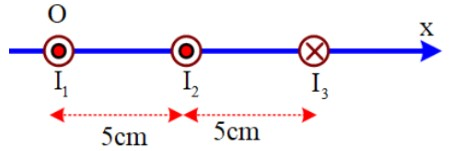
\includegraphics[width=0.4\linewidth]{../figs/VN12-Y24-PH-SYL-019P-8}
\end{center}
	\choice
	{\True $\SI{-5}{\centi\meter}$ và $\SI{4}{\centi\meter}$}
	{$\SI{-3}{\centi\meter}$ và $\SI{4.5}{\centi\meter}$}
	{$\SI{5}{\centi\meter}$ và $\SI{-4}{\centi\meter}$}
	{$\SI{3}{\centi\meter}$ và $\SI{-4.5}{\centi\meter}$}
	\loigiai{
Hướng cảm ứng từ gây ra bởi 3 dòng điện trong các miền lần lượt là:
$$\begin{cases}
	\text{Miền 1} \left(x<0\right): \vec{B}_1\downarrow\vec{B}_2\downarrow\vec{B}_3\uparrow\\
	\text{Miền 2} \left(0<x<\SI{0.05}{\meter}\right): \vec{B}_1\uparrow\vec{B}_2\downarrow\vec{B}_3\uparrow\\
	\text{Miền 3} \left(\SI{0.05}{\meter}<x<\SI{0.1}{\meter}\right): \vec{B}_1\uparrow\vec{B}_2\uparrow\vec{B}_3\uparrow\\
	\text{Miền 4} \left(x>\SI{0.1}{\meter}\right): \vec{B}_1\uparrow\vec{B}_2\uparrow\vec{B}_3\downarrow
\end{cases}	$$
Xét trường hợp nếu độ lớn cảm ứng từ tổng hợp trong miền 1 và miền 4 bằng 0 thì:
$$B_{\mathrm{M}}=2\cdot10^{-7}\left|\dfrac{I_1}{x}+\dfrac{I_2}{x-0,05}-\dfrac{I_3}{x-0,1}\right|=0\Rightarrow \hoac{x=\SI{0.04}{\meter}=\SI{4}{\centi\meter}}{
x=\SI{-0.05}{\meter}=\SI{-5}{\centi\meter}}.$$
}
\end{ex}


\Closesolutionfile{ans}

\section{Trắc nghiệm đúng/sai}
\Opensolutionfile{ans}[ans/VN12-Y24-PH-SYL-019P-TF]
\setcounter{ex}{0}
% ===================================================================
\begin{ex}\mkstar{3}
	Hai dây dẫn thẳng, dài vô hạn, mang dòng điện cùng chiều có cường độ lần lượt là $I_1=\SI{1}{\ampere}$ và $I_2=\SI{2}{\ampere}$ được đặt song song, cách nhau $\SI{10}{\centi\meter}$ trong không khí. Bỏ qua tác dụng của từ trường Trái Đất. Nhận định về các phát biểu sau đây.
	\choiceTF[t]
	{Hai dây dẫn sẽ đẩy nhau}
	{Từ trường do mỗi dây dẫn gây ra tại vị trí của dây dẫn kia có độ lớn cảm ứng từ bằng nhau}
	{\True Độ lớn lực từ do mỗi dây dẫn gây ra cho dây dẫn còn lại là bằng nhau}
	{\True Độ lớn lực từ do dây dẫn 1 gây ra cho dây dẫn 2 là $\SI{4E-6}{\micro\newton}$}
	\loigiai{}
\end{ex}


\Closesolutionfile{ans}
\section{Tự luận}
\setcounter{ex}{0}
\Opensolutionfile{ans}[ans/VN12-Y24-PH-SYL-019P-TL]
% ======================================================================
\begin{ex}\mkstar{2} 
Cho dây dẫn thẳng dài vô hạn có cường độ dòng điện $\SI{0.5}{\ampere}$ chạy qua.
\begin{enumerate}[label=\alph*)]
	\item Tính độ lớn cảm ứng từ tại điểm A cách dây dẫn một đoạn $\SI{4}{\centi\meter}$.
	\item Tính khoảng cách từ điểm $C$ đến dây dẫn, biết cảm ứng từ tại điểm $C$ có độ lớn $\SI{4E-6}{\tesla}$.	
\end{enumerate}
	\loigiai{
\begin{enumerate}[label=\alph*)]
	\item Độ lớn cảm ứng từ tại điểm A xác định bởi:
	$$
	B_{\mathrm{A}}=2 \cdot 10^{-7} \cdot\frac{I}{r_{\mathrm{A}}}=2 \cdot 10^{-7}\cdot \frac{0,5}{4.10^{-2}}=\SI{2.5E-6}{\tesla}.
	$$
	\item Từ công thức tính độ lớn cảm ứng từ tại điểm C, suy ra được khoảng cách từ điểm $C$ đến dây dẫn:
	$$
	B_{\mathrm{C}}=2 \cdot 10^{-7} \cdot\frac{I}{r_{\mathrm{C}}} \Rightarrow r_{\mathrm{C}}=2 \cdot 10^{-7}\cdot \frac{I}{B_{\mathrm{C}}}=2 \cdot 10^{-7}\cdot \frac{0,5}{4\cdot 10^{-6}}=\SI{2.5E-2}{\meter}=\SI{2.5}{\centi\meter}.
	$$
\end{enumerate}	
}
\end{ex}
% ======================================================================
\begin{ex}\mkstar{2}
	Một ống dây hình trụ được quấn bằng dây đồng có đường kính tiết diện $\SI{0.5}{\milli\meter}$. Biết rằng các vòng dây quấn sát nhau và che kín lõi của ống. Cường độ dòng điện chạy trong dây dẫn của ống có giá trị $\SI{50}{\milli\ampere}$. Hãy tính độ lớn cảm ứng từ bên trong ống dây.
	\loigiai{
Độ lớn cảm ứng từ bên trong ống dây là:
$$
B=4 \pi \cdot 10^{-7} \cdot\frac{N I}{L}=4 \pi \cdot 10^{-7} \cdot\frac{I}{d}=4 \pi \cdot 10^{-7} \cdot\frac{50 \cdot 10^{-3}}{0,5 \cdot 10^{-3}} \approx \SI{125.7}{\micro\tesla}.
$$	
}
\end{ex}
% ======================================================================
\begin{ex}\mkstar{3}
Máy chụp cộng hưởng từ MRI (Magnetic Resonance Imaging) là một trong những thiết bị hỗ trợ chẩn đoán hình ảnh những cơ quan bên trong cơ thể một cách chi tiết (Hình \ref{fig:19P-1}). Máy MRI có mức độ an toàn cao do không sử dụng các tia bức xạ như tia X. Máy MRI sử dụng một từ trường mạnh để tạo ra hình ảnh chất lượng cao của cấu trúc bên trong cơ thể như: não, xương, cơ và các mô khác.
\begin{center}
	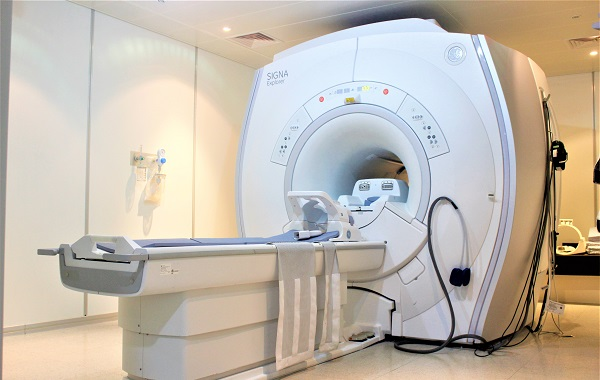
\includegraphics[width=0.4\linewidth]{../figs/VN12-Y24-PH-SYL-019P-1}
	\captionof{figure}{Máy chụp MRI}
	\label{fig:19P-1}
\end{center} 
Một máy MRI sử dụng từ trường có độ lớn cảm ứng từ là $\SI{1.5}{\tesla}$, có chiều dài khoảng $\SI{1.4}{\meter}$ và có đường kính $\SI{2.5}{\meter}$. Giả sử ta mô hình hoá máy MRI hoạt động như một cuộn dây dẫn mang dòng điện.
\begin{enumerate}[label=\alph*)]
	\item Hãy ước lượng số vòng dây cần thiết để tạo ra một từ trường có độ lớn cảm ứng từ $\SI{1.5}{\tesla}$ bên trong máy. Xem mỗi vòng dây có dòng điện với cường độ $\SI{100}{\ampere}$ chạy qua.
	\item Xác định điện trở của cuộn dây này. Biết rằng đối với dòng điện có cường độ $\SI{100}{\ampere}$, kích thước dây điển hình thường được sử dụng đối với chất liệu đồng là loại dây có chỉ số 2 AWG (chỉ số AWG - American Wire Gauge: chỉ số dùng để mô tả kích cỡ dây dẫn theo tiêu chuẩn Hoa Kỳ) với đường kính tiết diện tròn khoảng $\SI{6.54}{\milli\meter}$ và điện trở suất $\SI{1.69E-8}{\ohm\cdot\meter}$.
	\item Xác định nhiệt lượng toả ra trên dây dẫn này khi máy MRI làm việc một lần trong khoảng 30 phút (thời gian làm việc của máy còn tuỳ thuộc vào bộ phận cơ thể được chụp và số lượng hình ảnh cần thiết) và chi phí cần phải chi trả do hao phí năng lượng xuất hiện trên dây dẫn, biết rằng chi phí có giá trung bình khoảng $\SI{1600}{\text{đồng}/\kilo\watt\hour}$. Tìm hiểu về tính khả thi khi sử dụng mô hình xem máy MRI hoạt động như một cuộn dây dẫn mang dòng điện.
\end{enumerate}
	\loigiai{
	\begin{enumerate}[label=\alph*)]
		\item Số vòng dây mang dòng điện $\SI{100}{\ampere}$ để tạo ra một từ trường cần thiết bên trong máy MRI xác định bởi biểu thức:
		$$
		B=4 \pi \cdot 10^{-7} \cdot\frac{N I}{L} \Rightarrow N=\frac{B L}{4 \pi \cdot 10^{-7} I}=\frac{1,5 \cdot 1,4}{4 \pi \cdot 10^{-7} \cdot 100} \approx \SI{16711}{\text{vòng}}.
		$$
		\item Điện trở của cuộn dây dẫn điện xác định bởi biểu thức:
		$$
		R=\rho \frac{\ell}{S}=\frac{\rho N \pi d}{\pi\left(\frac{d_0}{2}\right)^2}=\frac{4 \rho N d}{d_0^2}=\frac{4 \cdot 1,69 \cdot 10^{-8} \cdot 16711 \cdot 2,5}{\left(6,54 \cdot 10^{-3}\right)^2} \approx \SI{66.03}{\ohm}.
		$$
		\item Công suất toả nhiệt của dây dẫn: $\mathcal{P}=I^2 \cdot R=100^2 \cdot 66,03=\SI{660.3}{\watt}$. Nhiệt lượng toả ra trên dây dẫn khi máy MRI làm việc trong 30 phút:
		$$
		Q=\mathcal{P} t=660,3 \cdot \frac{1}{2}=\SI{330.15}{\kilo\watt\hour}.
		$$
		Chi phí cần phải chi trả do nhiệt lượng toả ra trên dây dẫn này khi máy MRI làm việc một lần trong 30 phút là: $330,15.1600=528240$ đồng.\\
		\textbf{Nhận xét}: Công suất toả nhiệt trên dây dẫn theo mô hình này là quá lớn và không có ý nghĩa thực tiễn trong việc chế tạo. Trên thực tế, trong máy MRI, từ trường được tạo ra bởi nam châm siêu dẫn - một loại nam châm đặc biệt được làm từ vật liệu siêu dẫn, vật liệu này có đặc tính là có điện trở rất nhỏ khi được làm lạnh xuống gần độ không tuyệt đối - khoảng $\SI{10}{\kelvin}$ và cần được giữ ở nhiệt độ cực thấp để duy trì đặc tính siêu dẫn của nó.
	\end{enumerate}
}
\end{ex}
% ======================================================================
\begin{ex}\mkstar{3}
	Loa là một thiết bị có nhiệm vụ phát ra âm thanh bằng cách truyền tín hiệu điện thành tín hiệu âm thanh (sóng âm). Tín hiệu này làm không khí xung quanh loa dao động và truyền đến tai người nghe. Loa có thể được cấu tạo gồm các bộ phận đơn giản như hình \ref{fig:19P-2}a. Khi tín hiệu điện biến thiên theo tần số của tín hiệu âm thanh, cuộn dây và màng loa dao động cùng tần số, dẫn đến sự dao động của không khí và sóng âm được tạo ra.
	\begin{center}
			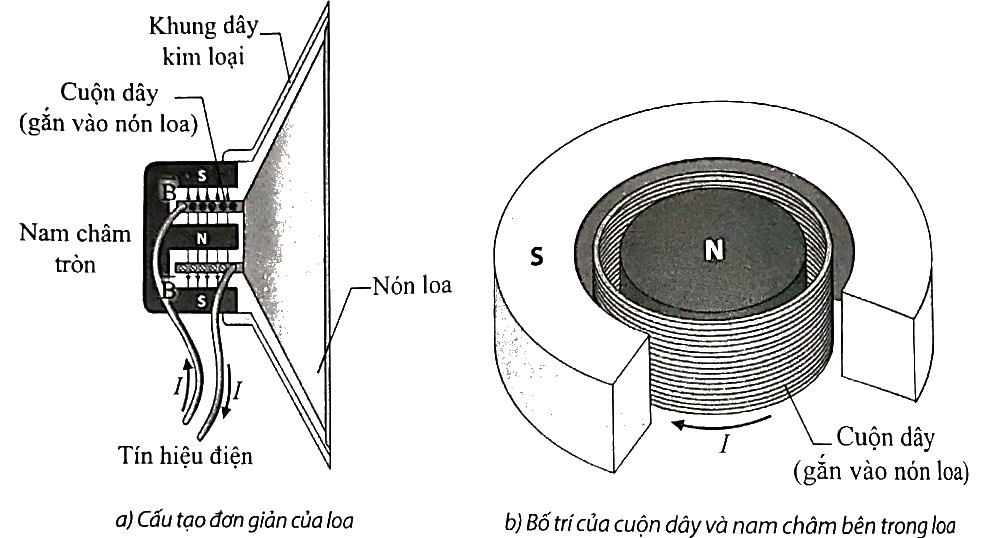
\includegraphics[width=0.65\linewidth]{../figs/VN12-Y24-PH-SYL-019P-2}
			\captionof{figure}{}
			\label{fig:19P-2}
	\end{center}
	Cấu tạo đơn giản của bộ phận tạo ra sự dao động của không khí của loa gồm hai phần: nam châm hình tròn được đặt cố định, trọng tâm nam châm đặt thẳng hàng với trọng tâm màng loa và cuộn dây hình tròn (Hình \ref{fig:19P-2}b). Khi dòng điện thay đổi theo thời gian chạy qua cuộn dây đặt trong từ trường của nam châm sẽ làm xuất hiện lực từ tác dụng lên cuộn dây, lực từ này có chiều thay đổi làm nón loa dao động theo, từ đó tạo ra âm thanh phát ra tương ứng với tín hiệu âm thanh đầu vào.\\
	Xét một loa điện có một cuộn dây nằm trong khe hở của một nam châm, giả sử từ trường của nam châm có độ lớn cảm ứng từ là $\SI{0.08}{\tesla}$. Cuộn dây có đường kính khoảng $\SI{6.4}{\centi\meter}$, gồm 18 vòng dây và có điện trở là $\SI{6.0}{\ohm}$. Khi kết nối với nguồn có hiệu điện thế $\SI{12}{\volt}$, dòng điện chạy trong cuộn dây tại một thời điểm xác định có chiều cùng chiều kim đồng hồ như hình \ref{fig:19P-2}b. Tại thời điểm này, xác định lực từ tác dụng trên cuộn dây.
	\loigiai{
	\begin{center}
		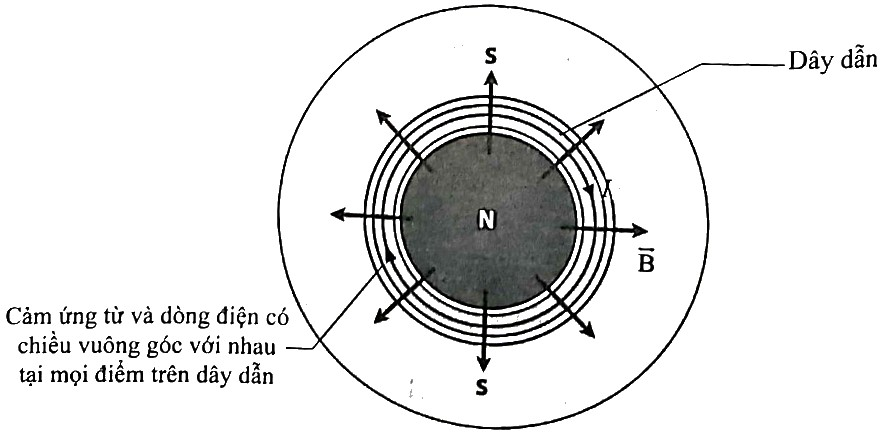
\includegraphics[width=0.6\linewidth]{../figs/VN12-Y24-PH-SYL-019P-3}
	\end{center}
Theo định luật Ohm, dòng điện chạy trong cuộn dây có cường độ là:
$$
I=\frac{U}{R}=\frac{12}{6}=\SI{2}{\ampere}
$$
Vì tại mọi điểm trên dây dẫn, từ trường song song với mặt phẳng vòng dây và vuông góc với chiều dòng điện nên lực từ tác dụng lên cuộn dây có phương vuông góc với mặt phẳng hình vẽ, có độ lớn xác định tương tự như đặt một đoạn dây thẳng có cùng chiều dài $L$ với cuộn dây trong từ trường, trong đó $L=N \pi d=18 \cdot \pi \cdot 6,4 \approx \SI{3.62}{\meter}$.\\
Khi đó lực từ tác dụng lên cuộn dây có phương vuông góc với mặt phẳng hình vẽ và chiều hướng ra ngoài (xác định bằng quy tắc bàn tay trái) và có độ lớn là:
$$
F=B I L=0,08 \cdot 2 \cdot 3,62 \approx \SI{0.58}{\newton}.
$$
}
\end{ex}











\Closesolutionfile{ans}
